% !TEX root = ../intrinsic_offline_RL_bound_arxiv.tex


As a step towards the optimal and strong adaptive offline RL bound, we analyze \emph{the vanilla pessimistic value iteration} (VPVI), a tabular counterpart of \emph{pessimistic value iteration} (PEVI initiated in \cite{jin2020pessimism}), to understand what is missing for achieving the fully adaptivity. In particular, VPVI relies on the model-based construction.



\textbf{Model-based Components.} Given data {\small$\mathcal{D}=\left\{\left(s_{h}^{\tau}, a_{h}^{\tau}, r_{h}^{\tau}, s_{h+1}^{\tau}\right)\right\}_{\tau\in[n]}^{h \in[H]}$}, we denote $n_{s_h,a_h}:=\sum_{\tau=1}^n\mathbf{1}[s_h^{\tau},a_h^{\tau}=s_h,a_h]$ be the total counts that visit $(s_h,a_h)$ pair at time $h$, then we use the offline plug-in estimator to construct the estimators for ${P_h}$ and $r_h$ as:
{\small
\begin{equation}\label{eqn:mb_est}
\widehat{P}_h(s'|s_h,a_h)=\frac{\sum_{\tau=1}^n\mathbf{1}[(s^{\tau}_{h+1},a^{\tau}_h,s^{\tau}_h)=(s^\prime,s_h,a_h)]}{n_{s_h,a_h}},\; \widehat{r}_h(s_h,a_h)=\frac{\sum_{\tau=1}^n\mathbf{1}[(a^{\tau}_h,s^{\tau}_h)=(s_h,a_h)]\cdot r_h^\tau}{n_{s_h,a_h}},
\end{equation}
}if $n_{s_h,a_h}>0$ and $\widehat{P}_h(s'|s_h,a_h)={1}/{S},\widehat{r}_h(s_h,a_h)=0$ if $n_{s_h,a_h}=0$. In particular, we use the word ``vanilla'' as it directly mirrors \cite{jin2020pessimism} with a pessimistic penalty of order $O(H/\sqrt{n_{s_h,a_h}})$.\footnote{This is due to $\sqrt{\phi\left(s_{h}, a_{h}\right)^{\top} \Lambda_{h}^{-1} \phi\left(s_{h}, a_{h}\right)}$ reduces to $\sqrt{{1}/n_{s_h,a_h}}$ when setting $\phi(s_h,a_h)=\mathbf{1}(s_h,a_h)$ and $\lambda=0$.} With $\widehat{P}_h,\widehat{r}_h$ in Algorithm~\ref{alg:VPVI} (which we defer to Appendix), VPVI guarantees the following:



\begin{theorem}\label{thm:VPVI}
Under the Assumption~\ref{assum:single_concen}, denote $\bar{d}_m:=\min_{h\in[H]}\{d^\mu_h(s_h,a_h):d^\mu_h(s_h,a_h)>0\}$. For any $0<\delta<1$, there exists absolute constants $c_0,C'>0$, such that when $n>c_0 \cdot 1/\bar{d}_m\cdot\iota$ ($\iota=\log(HSA/\delta)$), with probability $1-\delta$, the output policy $\widehat{\pi}$ of VPVI satisfies
{
\begin{equation}\label{eqn:VPVI}
0\leq v^\star-v^{\widehat{\pi}}\leq C'H\sum_{h=1}^H\sum_{(s_h,a_h)\in\mathcal{C}_h}d^{\pi^\star}_h(s_h,a_h)\cdot\sqrt{\frac{\iota}{ n\cdot d^\mu_h{(s_h,a_h)}}}.
\end{equation}
}
\end{theorem}
The full proof can be found in Appendix~\ref{sec:VPVI_proof}. Theorem~\ref{thm:VPVI} makes some improvements over the existing works. First, it is more adaptive than the results with uniform data-coverage Assumption~\ref{assum:uniform} (\cite{yin2021near,ren2021nearly}). In addition, by straightforward calculation \eqref{eqn:VPVI} can be bounded by $\tilde{O}(\sqrt{H^4SC^\star/n})$ which improves VI-LCB \citep{rashidinejad2021bridging} by a factor of $H$.\footnote{To be rigorous, translating the result from the infinite horizon setting to the finite horizon setting requires explanation. We add this discussion in Appendix~\ref{sec:dis_VPVI}.} Besides, the analysis of VPVI also improves the direct reduction of PEVI \citep{jin2020pessimism} in the tabular case by a factor $SA$ since their $\beta=SAH$ when $d=SA$.  

However, VPVI is not optimal as the dependence on horizon is $H^4$ which does not match the optimal worst case guarantee $H^3$ \citep{yin2021near} in the nonstationary setting. Also, the explicit dependence on $H$ in \eqref{eqn:VPVI} possibly hides some key features of the specific offline RL instances. For example, no improvement can be made if the system has the deterministic transition.
	
	
 








\begin{algorithm}[H]
	\caption{Adaptive (\emph{assumption-free}) Pessimistic Value Iteration or LCBVI-Bernstein}
	\label{alg:APVI}
	\small{
		\begin{algorithmic}[1]
			\STATE {\bfseries Input:} Offline dataset $\mathcal{D}=\{(s_h^\tau,a_h^\tau,r_h^\tau,s_{h+1}^\tau)\}_{\tau,h=1}^{n,H}$. Set $C_1=2,C_2=14$, failure probability $\delta$.
			
			\STATE {\bfseries Initialization:} Set $\widehat{V}_{H+1}(\cdot)\leftarrow 0$.  Set $\iota=\log(HSA/\delta)$. (if assumption-free, set $M^\dagger,\widehat{M}^\dagger$ as in Section~\ref{sec:assumption_free}.)
			
			\FOR{time $h=H,H-1,\ldots,1$}
			\STATE Set $\widehat{Q}_h(\cdot,\cdot)\leftarrow {\widehat{r}_h(\cdot,\cdot)}+(\widehat{P}_{h}\cdot \widehat{V}_{h+1})(\cdot,\cdot)$\;\;(use ${\widehat{r}_h^\dagger}+(\widehat{P}_{h}^\dagger\cdot \widehat{V}_{h+1})$ if assumption-free)
			\STATE $\forall s_h,a_h$, set $\Gamma_h(s_h,a_h)=C_1\sqrt{\frac{\mathrm{Var}_{\widehat{P}_{s_h,a_h}}(\widehat{r}_h+\widehat{V}_{h+1})\cdot\iota}{n_{s_h,a_h}}}+\frac{C_2H\cdot\iota}{n_{s_h,a_h}}$ if $n_{s_h,a_h}\geq 1$, o.w. set to $\frac{CH\iota}{1}$. 
			 \STATE (If assumption-free, use $C_1\sqrt{{\mathrm{Var}_{\widehat{P}^\dagger_{s_h,a_h}}(\widehat{r}^\dagger_h+\widehat{V}_{h+1})\cdot\iota}/{n_{s_h,a_h}}}+\frac{C_2H\cdot\iota}{n_{s_h,a_h}}$ if $n_{s_h,a_h}\geq 1$, o.w. use $0$.)
			\STATE Set $\widehat{Q}^p_h(\cdot,\cdot)\leftarrow \widehat{Q}_h(\cdot,\cdot)-\Gamma_h(\cdot,\cdot)$.   Set $\overline{Q}_h(\cdot,\cdot)\leftarrow \min\{\widehat{Q}^p_h(\cdot,\cdot),H-h+1\}^{+}$.\COMMENT{Pessmistic update}
			\STATE $\forall s_h$, Select $\widehat{\pi}_h(\cdot|s_h)\leftarrow \argmax_{\pi_h}\langle \overline{Q}_h(s_h,\cdot),\pi_h(\cdot|s_h)\rangle$. Set $\widehat{V}_h(s_h)\leftarrow\langle \overline{Q}_h(s_h,\cdot), \widehat{\pi}_h(\cdot|s_h) \rangle$.
			\ENDFOR
			
			\STATE {\bfseries Output: $\{\widehat{\pi}_h\}$. } 
			
		\end{algorithmic}
	}
\end{algorithm}

\section{Intrinsic Offline Reinforcement Learning bound}\label{sec:intrinsic}

Now we go deeper to understand what is the more intrinsic characterization for offline reinforcement learning. From the study of VPVI, penalizing the Q-function by $\widetilde{O}(H/\sqrt{n_{s_h,a_h}})$ is crude as it estimates the confidence width of $\widehat{Q}_h$ in Algorithm~\ref{alg:VPVI} too conservatively therefore loses the accuracy (the bound is suboptimal). This motivates us to use empirical standard deviation instead to create a more adaptive (and also less conservative) Bernstein-type confidence width as the pessimistic penalty:
{\small
 \begin{equation}\label{eqn:pessimistic_pen}
\Gamma_h(s_h,a_h)=\widetilde{O}\bigg[\sqrt{\frac{\mathrm{Var}_{\widehat{P}_{s_h,a_h}}(\widehat{r}_h+\widehat{V}_{h+1})}{n_{s_h,a_h}}}+\frac{H}{n_{s_h,a_h}}\bigg]\;(\text{if} \;n_{s_h,a_h}>0);\;=\widetilde{O}(H)\;(\text{if} \;n_{s_h,a_h}=0).
\end{equation}
}and update $\widehat{Q}_h\leftarrow\widehat{Q}_h-\Gamma_h$. On one hand, $\sqrt{{\mathrm{Var}_{\widehat{P}_{s_h,a_h}}(\widehat{r}_h+\widehat{V}_{h+1})}/{n_{s_h,a_h}}}$ is a ``less pessimistic'' penalty than VPVI due to $\sqrt{\mathrm{Var}_{\widehat{P}}(\widehat{r}_h+\widehat{V}_{h+1})}\leq H$ and critically this design is more data-adaptive since it holds negative view towards the locations with high uncertainties and recommends the locations that we are confident about, as opposed to the online RL (which encourages exploration in the uncertain locations). Such principles are not reflected by the isotropic design in VPVI. On the other hand, it carries the extremely negative view towards fully agnostic locations $\widetilde{O}(H)$ which in turn causes the agent unlikely to choose them. We summarized the this \emph{adaptive pessimistic value iteration} (APVI) into the Algorithm~\ref{alg:APVI}, with $\widehat{P}_h,\widehat{r}_h$ defined in \eqref{eqn:mb_est}. APVI has the following guarantee. A sketch of the analysis is presented in Section~\ref{sec:proof_sketch} and Appendix~\ref{sec:proof_APVI} includes the full proof. 





\begin{theorem}[Intrinsic offline RL bound]\label{thm:APVI}
	Under the Assumption~\ref{assum:single_concen}, denote $\bar{d}_m:=\min_{h\in[H]}\{d^\mu_h(s_h,a_h):d^\mu_h(s_h,a_h)>0\}$. For any $0<\delta<1$, there exists absolute constants $c_0,C'>0$, such that when $n>c_0 \cdot 1/\bar{d}_m\cdot\iota$ ($\iota=\log(HSA/\delta)$), with probability $1-\delta$, the output policy $\widehat{\pi}$ of APVI (Algorithm~\ref{alg:APVI}) satisfies ($\widetilde{O}$ hides log factor and higher order terms)
	\begin{equation}\label{eqn:APVI}
	0\leq v^\star-v^{\widehat{\pi}}\leq C'\sum_{h=1}^H\sum_{(s_h,a_h)\in\mathcal{C}_h}d^{\pi^\star}_h(s_h,a_h)\cdot\sqrt{\frac{\mathrm{Var}_{P_{s_h,a_h}}(r_h+V^\star_{h+1})\cdot\iota}{ n\cdot d^\mu_h{(s_h,a_h)}}}+\widetilde{O}\left(\frac{H^3}{n\cdot \bar{d}_m}\right)
	\end{equation}
\end{theorem}
\begin{remark}
	APVI (Algorithm~\ref{alg:APVI}) can also be called \textbf{LCBVI-Bernstein} as it creates the offline counterpart of UCBVI in \cite{azar2017minimax}. However, to highlight that the resulting bound fully adapts to the specific system structure, we use the word ``adaptive'' instead.
\end{remark}


APVI makes significant improvements in a lot of aspects. First and foremost, the dominate term is fully expressed by the system quantities that admits no explicit dependence on $H,S,A$. To the best of our knowledge, this is the first offline RL bound that concretely depicts the interrelations within the problem when the problem instance is a tuple $(M,\pi^\star,\mu)$: an MDP $M$ (coupled with the optimal policy $\pi^\star$) with the data rolling from an offline logging policy $\mu$. As we will discuss later, this result indicates (nearly) all the optimal worst-case non-adaptive bounds (and clearly also the VPVI) under their respective regimes / assumptions. Thus, \eqref{eqn:APVI} is generic. More interestingly, Theorem~\ref{thm:APVI} caters to the specific MDP structures and adaptively yields improved sample complexities (\emph{e.g.} faster convergence in deterministic systems) that existing works cannot imply. Such features are crucial as it helps us to understand what type of problems are harder / easier than others, and even more, in a \emph{quantitative} way. Last but not least, to illustrate this bound exhibits the intrinsic nature of offline RL, we prove a \emph{per-instance dependent} information-theoretical lower bound that shares a similar formulation. The proof of Theorem~\ref{thm:adaptive_lower_bound} can be found in Appendix~\ref{sec:proof_lower_bound}. 


\begin{theorem}[Instance-dependent information theoretical offline lower bound]\label{thm:adaptive_lower_bound}
	Denote $\mathcal{G}:=\{(\mu,M): \exists \pi^\star\;s.t. \; d^\mu_h(s,a)>0\;\text{if}\;d^{\pi^\star}_h(s,a)>0\}$. Fix an instance $\mathcal{P}=(\mu,M)\in\mathcal{G}$. Let $\mathcal{D}$ consists of $n$ episodes and define $\xi=\sup_{h,s_h,a_h,s_{h+1}, d^\mu_h(s_h,a_h)\cdot \Var_{P_{s_h,a_h}}(V_{h+1}^\star)>0}\frac{P_h(s_{h+1}|s_h,a_h)\left(V_{h+1}^\star(s_{h+1})-\E_{P_{s_h,a_h}}[V_{h+1}^\star]\right)}{\sqrt{2\cdot  d^\mu_h(s_h,a_h)\cdot \Var_{P_{s_h,a_h}}(V_{h+1}^\star)}}$. Let $\widehat{\pi}$ to be the output of any algorithm.  Define the {local non-asymptotic minimax risk} as 
	\begin{equation}\label{eqn:local_risk}
	\mathfrak{R}_{n}(\mathcal{P}):=\sup_{\mathcal{P}'\in\mathcal{G}}\inf_{\widehat{\pi}}\max_{\mathcal{Q}\in\{\mathcal{P},\mathcal{P}'\}}\sqrt{n}\cdot\E_{\mathcal{Q}}\left[v^\star(\mathcal{Q})-v^{\widehat{\pi}}\right]
	\end{equation}
	where $v^\star(\mathcal{Q})$ denotes the optimal value under the instance $\mathcal{Q}$. Then there exists universal constants $c_0,p,C>0$, such that if $n\geq c_0{H^6\xi^4}/{(\sum_{h=1}^H \sum_{s_h,a_h}d^{\pi^\star}_h(s_h,a_h)\sqrt{\frac{\Var_{P_{s_h,a_h}}(V_{h+1}^\star)}{ \zeta \cdot d^\mu_h(s_h,a_h)}})^2}$, with constant probability $p>0$, 
	Then we have (here $\zeta =H/\bar{d}_m$):
	\begin{equation}\label{eqn:lower}
	\mathfrak{R}_{n}(\mathcal{P})\geq C\cdot {\sum_{h=1}^H\sum_{(s_h,a_h)\in\mathcal{C}_h}d^{\pi^\star}_h(s_h,a_h)\cdot\sqrt{\frac{\mathrm{Var}_{P_{s_h,a_h}}(r_h+V^\star_{h+1})}{\zeta \cdot d^\mu_h{(s_h,a_h)}}}},
	\end{equation}
	where $\mathcal{P}=(\mu,M)$ and $M=(\mathcal{S}, \mathcal{A}, P, r, H, d_1)$.
\end{theorem}

The interpretation of Theorem~\ref{thm:adaptive_lower_bound} is: for any instance $\mathcal{P}$, learning requires \eqref{eqn:lower} (divided by $1/\sqrt{n}$) for any algorithm. Note this notion is significantly stronger than the previous minimax offline lower bounds \citep{yin2021near,rashidinejad2021bridging,xie2021policy,jin2020pessimism} (where they only select a particular family of hard problems), therefore, their lower bounds in general do not hold for individual instances. 

The quantity \eqref{eqn:intrinsic} nearly-matches the per-instance lower bound \eqref{eqn:lower} (they deviate by a factor of $\zeta=H/\bar{d}_m$ due to the technical reason) and, in addition, we provide a matching minimax lower bound in Appendix~\ref{sec:minimax_lower}. These results certify Theorem~\ref{thm:APVI} is not only adaptive but also near-optimal. Hence, we call the quantity $\sum_{h=1}^H\sum_{(s_h,a_h)\in\mathcal{C}_h}d^{\pi^\star}_h(s_h,a_h)\cdot\sqrt{\frac{\mathrm{Var}_{P_{s_h,a_h}}(r_h+V^\star_{h+1})}{ n\cdot d^\mu_h{(s_h,a_h)}}}$ \emph{intrinsic offline reinforcement learning bound}. In the sequel, we provide thorough discussions to explain the intrinsic bound embraces the fundamental challenges in offline RL and the strong adaptivity. The detailed technical derivations that are missing in Section~\ref{subsec:one}-\ref{subsec:three} are deferred to Appendix~\ref{sec:missing_dev}.



\begin{figure}[H]
	\centering     %%% not \center
	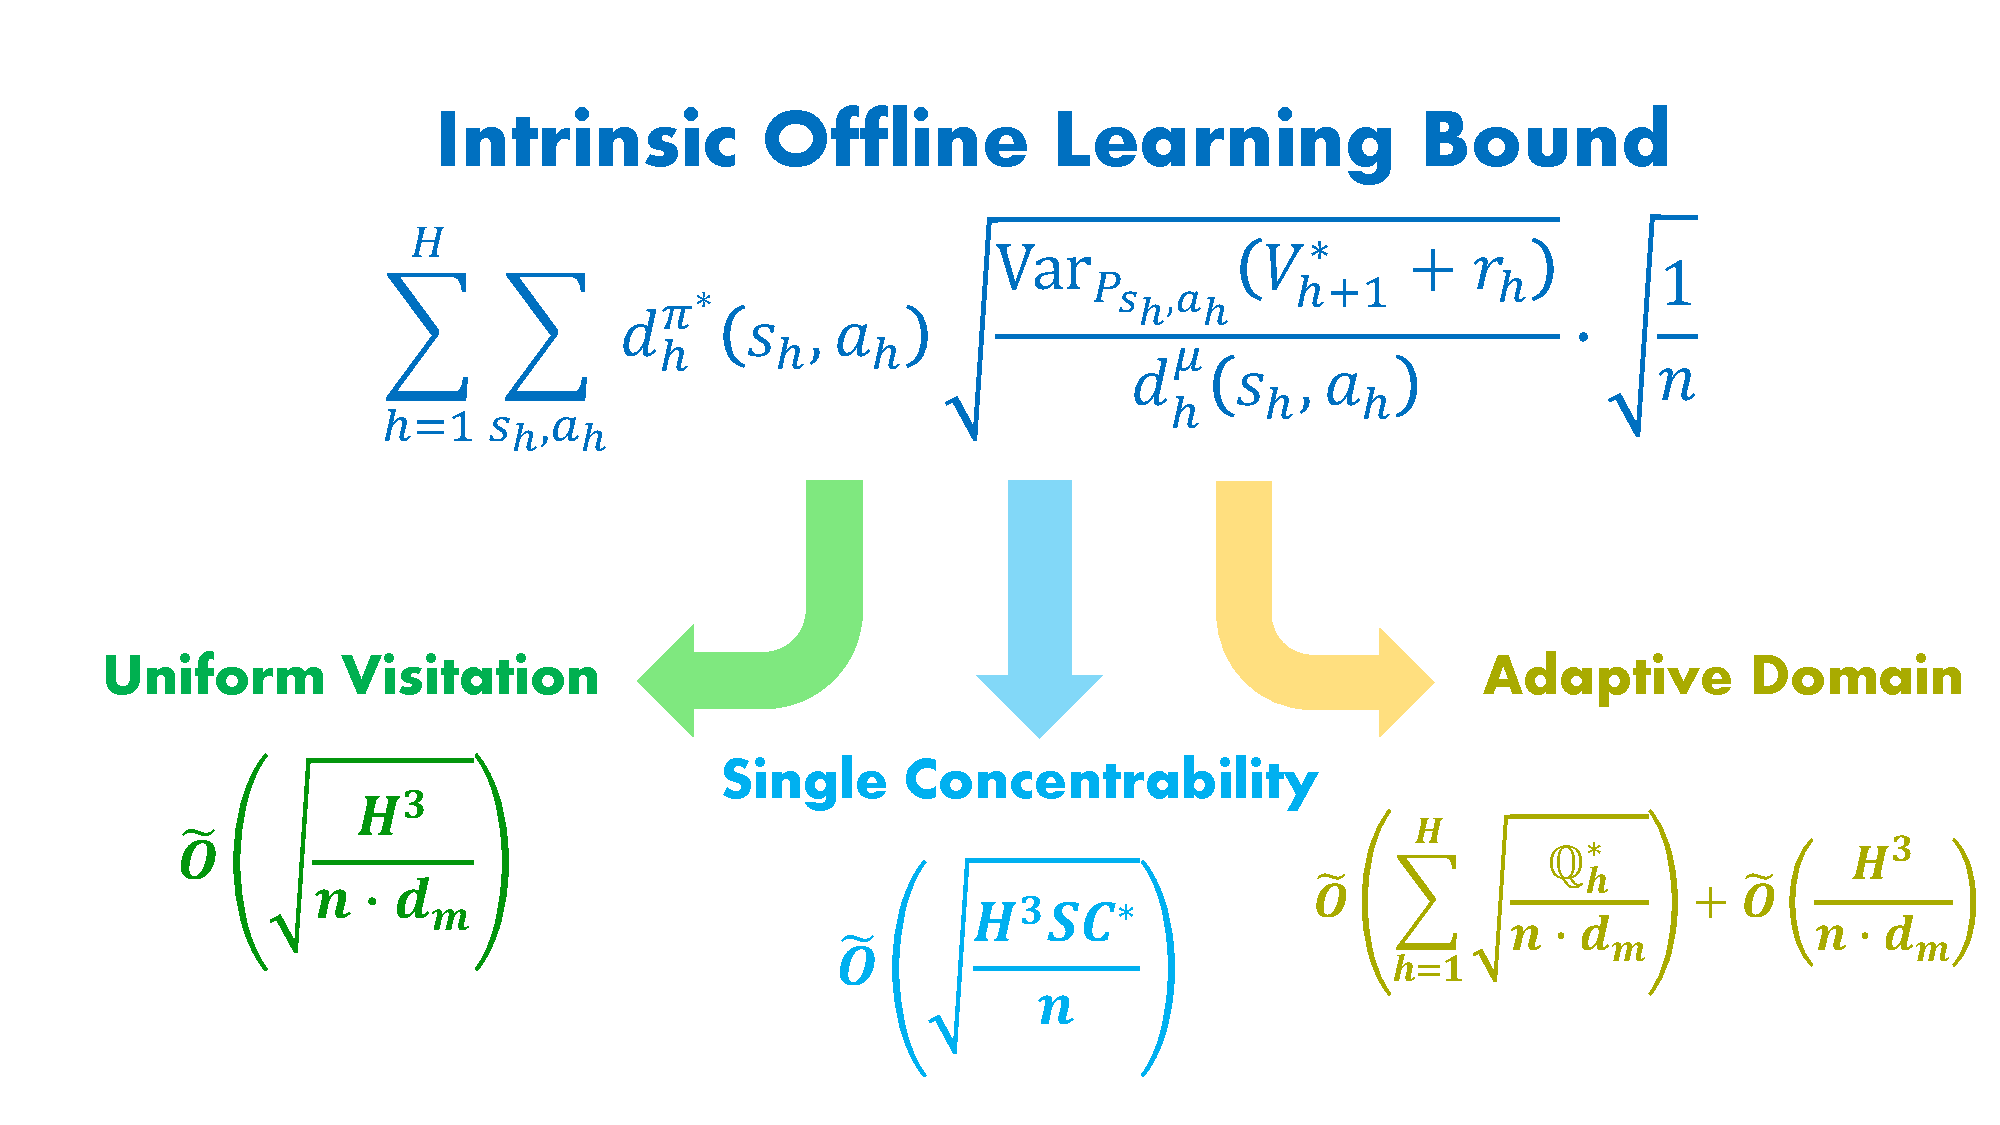
\includegraphics[width=115mm]{IOLB.pdf}
	\caption{A visualization on how intrinsic learning bound subsumes existing best-known results: uniform visitation, single concentrability (partial coverage) and adaptive domain.}
	\label{fig:main}
\end{figure}



\subsection{Optimality under Uniform data-coverage assumption}\label{subsec:one}

Under the uniform exploration Assumption~\ref{assum:uniform} with parameter $d_m:=\min_{h,s_h,a_h} d_h^\mu (s_h,a_h) > 0$, \cite{yin2021near} analyzes the model-based plug-in approach and obtains the optimal sample complexity $\widetilde{O}(H^3/d_m\epsilon^2)$ and shows $\Omega(H^3/d_m\epsilon^2)$ is also the lower bound. Indeed, this rate can be directly implied by the intrinsic RL bound via \emph{Cauchy inequality} and \emph{the Sum of Total Variance} (Lemma~\ref{lem:H3toH2}):\footnote{Here $\odot$ denotes element-wise multiplication. Also note under \ref{assum:uniform}, our $\bar{d}_m=d_m$.}
{\small
\begin{equation}\label{eqn:inter_derivation}
\begin{aligned}
&\sum_{h=1}^H\langle d^{\pi^\star}_h(\cdot),\sqrt{\frac{\mathrm{Var}_{P_{(\cdot)}}(r_h+V^\star_{h+1})}{ n\cdot d^\mu_h{(\cdot)}}}\rangle = \sum_{h=1}^H\langle \sqrt{d^{\pi^\star}_h(\cdot)},\sqrt{\frac{d^{\pi^\star}_h(\cdot)\odot\mathrm{Var}_{P_{(\cdot)}}(r_h+V^\star_{h+1})}{ n\cdot d_m}}\rangle\\
\leq &\sum_{h=1}^H\norm{ \sqrt{d^{\pi^\star}_h(\cdot)}}_2\norm{\sqrt{\frac{d^{\pi^\star}_h(\cdot)\odot\mathrm{Var}_{P_{(\cdot)}}(r_h+V^\star_{h+1})}{ n\cdot d_m}}}_2\leq \sqrt{\frac{H\cdot \mathrm{Var}_{\pi^\star}(\sum_{h=1}^{H} r_{h})}{n\cdot d_m}}\leq \sqrt{\frac{H^3}{n\cdot d_m}}
\end{aligned}
\end{equation}
}which translates to $\widetilde{O}(H^3/d_m\epsilon^2)$  complexity. Our result maintains the optimal worst-case guarantee when $\mu$ has the uniform data-coverage:

\begin{proposition}
	Under Assumption~\ref{assum:uniform} and apply Theorem~\ref{thm:APVI}, APVI achieves the sample complexity of minimax-rate $\widetilde{O}(H^3/d_m\epsilon^2)$ (Theorem~4.1 and Theorem~G.2 in \cite{yin2021near}).
\end{proposition}

\begin{remark}\label{remark:time-variant}
	We believe if the MDP is time-invariant, then by a modified construction of $\widehat{P}$, $\widehat{r}$ in \eqref{eqn:mb_est} our result will imply the minimax-rate of $\widetilde{O}(H^2/d_m\epsilon^2)$ as achieved in \cite{yin2021nearoptimal}. We include this discussion in Appendix~\ref{sec:missing_dev}.
\end{remark}

\subsection{Bounded sum of total rewards and the Horizon-Free case}\label{subsec:btr}
There is another thread of studies that follow the bounded sum of total rewards assumption: \emph{i.e.} $r_h\geq 0$, $\sum_{h=1}^H r_h\in [0,1]$ \citep{krishnamurthy2016pac,jiang2017contextual,zhang2020reinforcement}. Such a setting is much weaker than the uniform bounded instantaneous reward condition, as explained in \cite{jiang2018open}. In offline RL, \cite{ren2021nearly} derives the nearly horizon-free worst case bound $\widetilde{O}(\sqrt{1/nd_m})$ for the time-invariant MDPs, under the Assumption~\ref{assum:uniform}. As a comparison, our Theorem~\ref{thm:APVI} achieves the following guarantee for the time-varying (non-stationary) MDPs.

\begin{proposition}
	Assume $r_h\geq 0$, $\sum_{h=1}^H r_h\leq 1$. Then in the time-varying case AVPI (Theorem~\ref{thm:APVI}) outputs a policy $\widehat{\pi}$ such that the suboptimality gap $v^\star-v^{\widehat{\pi}}$ is bounded by $\widetilde{O}(\sqrt{H/nd_m})$ with high probability under the Assumption~\ref{assum:uniform}. 
\end{proposition}   

The derivation is straightforward by using $\mathrm{Var}_{\pi^\star}(\sum_{h=1}^{H} r_{h})\leq 1$ in \eqref{eqn:inter_derivation}. This proposition is interesting since it indicates when the MDP is non-stationary, $\widetilde{O}(H/d_m\epsilon^2)$ is required in the worst case even under $\sum_{h=1}^H r_h\leq 1$.\footnote{Suppose in this case we can achieve $\widetilde{O}(1/d_m\epsilon^2)$ just like \cite{ren2021nearly}, then by a rescaling we obtain the $\widetilde{O}(H^2/d_m\epsilon^2)$ under the usual $0\leq r_h\leq 1$ assumption which violates the $\Omega(H^3/d_m\epsilon^2)$ lower bound.} The extra $H$ factor resembles the challenge that we have $H$ transitions ($P_1,\ldots,P_H$) to learn, as opposed to the bandit-type $1/d_m\epsilon^2$ result due to there is only one $P$ throughout (time-invariant). This reveals that one hardness in solving the MDP is in proportion to the number of different transition kernels within the MDP. Such a finding could help researchers understand the special settings like \emph{low switching cost in transitions} \citep{bai2019provably} or \emph{non-stationarity} \citep{cheung2020reinforcement}.

\subsection{Optimality with Single Concentrability}\label{subsec:two}

In the finite horizon discounted setting, \cite{rashidinejad2021bridging} proposes the single policy concentrability assumption which is defined as $C^\star:=\max_{h,s,a}\frac{d^{\pi^\star}_h(s,a)}{d^\mu_h(s,a)}<\infty$ in the current episodic non-stationary MDP setting. As discussed in Appendix~\ref{sec:dis_VPVI}, their lower bound translates to $\Omega(\sqrt{\frac{H^3SC^\star}{n}})$ and their VI-LCB algorithm yields $\widetilde{O}(\sqrt{\frac{H^5SC^\star}{n}})$ suboptimality gap in $H$-horizon case. Since single policy concentrability is strictly weaker than its uniform version (Assumption~\ref{assum:concen}), we only discuss this set up. In particular, we have the following implication from our Theorem~\ref{thm:APVI} (whose derivation can be found in Appendix~\ref{sec:missing_dev}):

\begin{proposition}
	Let $\pi^\star$ be a deterministic policy such that $C^\star:=\max_{h,s,a}\frac{d^{\pi^\star}_h(s,a)}{d^\mu_h(s,a)}<\infty$. Then by Theorem~\ref{thm:APVI}, with high probability the output policy of APVI satisfies the suboptimality gap $\widetilde{O}(\sqrt{\frac{H^3SC^\star}{n}})$ in the time-varying (non-stationary) MDPs. 
\end{proposition}
This can computed similar to \eqref{eqn:inter_derivation} except we use $\frac{d^{\pi^\star}_h(s,a)}{d^\mu_h(s,a)}\leq C^\star$. Our implication improves the VI-LCB by the factor $H^2$ (in terms of sample complexity) and is optimal (recover the concurrent \cite{xie2021policy}). Qualitatively, single concentrability is the same as Assumption~\ref{assum:single_concen}, but the use of $C^\star$ makes the bound highly problem independent and limits the adaptivity. Problem dependent bound is a more interesting domain as it tailors to each MDP separately. We discuss it now.



\subsection{Problem dependent domain}\label{subsec:three}

We define the \emph{pre-step environmental norm} (the finite horizon counterpart of \cite{maillard2014hard}) as: $\mathbb{Q}^\star_h=\max_{s_h,a_h}\mathrm{Var}_{P_{s_h,a_h}}(r_h+V^\star_{h+1})$ for all $h\in[H]$, and relax the total sum of rewards to be bounded by any arbitrary value $\mathcal{B}$ (\emph{i.e.} $\sum_{h=1}^H r_h\leq \mathcal{B}$), then Theorem~\ref{thm:APVI} implies:
\begin{proposition}\label{prop}
	Under Assumption~\ref{assum:uniform}, with high probability, subopmality of AVPI is bounded by 
	{
	\[
	\min\left\{\widetilde{O}\big(\sum_{h=1}^H\sqrt{\frac{\mathbb{Q}^\star_h}{n\bar{d}_m}}\big),\widetilde{O}\big(\sqrt{\frac{H\cdot \mathcal{B}^2}{n\bar{d}_m}}\big)\right\}+\widetilde{O}(\frac{H^3}{n\bar{d}_m}).
	\]}  
\end{proposition} 
Such a result mirrors the online version of the tight problem-dependent bound \cite{zanette2019tighter} but with a more general \emph{pre-step environmental norm} for the non-stationary MDPs.\footnote{\cite{zanette2019tighter} uses the maximal version by maximizing over $h$.} For the problem instances with either small $\mathcal{B}$ or small $\mathbb{Q}_h^\star$, our result yields much better performances, as discussed in the following.

\textbf{Deterministic systems.} For many practical applications of interest, the systems are equipped with low stochasticity, \emph{e.g.} robotics, or even deterministic dynamics, \emph{e.g.} the game of GO. In those scenarios, the agent needs less experience for each state-action therefore the learning procedure could be much faster. In particular, when the system is fully deterministic (in both transitions and rewards) then $\mathbb{Q}^\star_h=0$ for all $h$. This enables a faster convergence rate of order $\frac{H^3}{n\bar{d}_m}$ and significantly improves over the existing non-adaptive results that have order $\frac{1}{\sqrt{n}}$. The convergence rate $\frac{1}{n}$ matches \cite{wen2013efficient} by translating their constant (in $T$) regret into the PAC bound.

\textbf{Partially deterministic systems.} Practical worlds are complicated and we could sometimes have a mixture model which contains both deterministic and stochastic steps. In those scenarios, the main complexity is decided by the number of stochastic stages: suppose there are $t$ stochastic $P_h,r_h$'s and $H-t$ deterministic $P_{h'},r_{h'}$'s, then completing the offline learning guarantees {\small$t\cdot\sqrt{{\max Q^\star_h}/{n \bar{d}_m}}$} suboptimality gap, which could be much smaller than {\small$H\cdot\sqrt{{\max Q^\star_h}/{n \bar{d}_m}}$} when $t\ll H$. 

\textbf{Fast mixing domains.} Consider a class of highly mixing non-stationary MDPs (a variant of \cite{zanette2018problem}) that satisfies the transition $P_h(\cdot|s_h,a_h):=\nu_h(\cdot)$ depends on neither the state $s_h$ nor the action $a_h$. Define $\bar{s}_{t} := \arg \max V_{t}^{\star}(s)$ and $\underline{s}_{t} := \arg \max V_{t}^{\star}(s)$. Also, denote $\mathrm{rng}V^\star_h$ to be the range of $V^\star_h$.
In such cases, Bellman optimality equations have the form
{
\[
V_{h}^{\star}\left(\bar{s}_{h}\right)=\max _{a}\left(r_h\left(\bar{s}_{h}, a\right)+\nu_h^{\top} V_{h+1}^{\star}\right),\;\;V_{h}^{\star}\left(\underline{s}_{h}\right)=\max _{a}\left(r_h\left(\underline{s}_{h}, a\right)+\nu_h^{\top} V_{h+1}^{\star}\right),
\]
}which yields $\mathrm{rng}V^\star_h=V_{h}^{\star}\left(\bar{s}_{h}\right)-V_{h}^{\star}\left(\underline{s}_{h}\right)=\max_ar_h\left(\bar{s}_{h}, a\right)-\min_ar_h\left(\underline{s}_{h}, a\right)\leq 1$, and this in turn gives $\mathbb{Q}_h^\star\leq 1+(\mathrm{rng}V^\star_h)^2=2$. As a result, the suboptimality is bounded by $\widetilde{O}(\sqrt{H^2/nd_m})$ in the worst case. This result reveals, although this is a family of stochastic non-stationary MDPs, but it is only as hard as the family of stationary MDPs in the minimax sense ($\Omega(H^2/d_m\epsilon^2)$).

\textbf{Tabular contextual bandits.} Our result also implies $\widetilde{O}(\sum_{x_1,a_1}d^{\pi^\star}_1(x_1,a_1)\sqrt{\frac{\mathrm{Var}{(r_1)}}{n\cdot d^\mu_1(x_1,a_1)}})$ gap for the \emph{offline tabular contextual bandit} problem and improves to $\widetilde{O}(1/nd_m)$ when the reward is deterministic. In either cases, the result is optimal and this is due to: when $r_1$ is deterministic, the agent only needs one sample at every location (see \cite{bubeck2012regret} for a survey).


















\section{Towards Assumption-Free Offline RL}\label{sec:assumption_free}
While assumption~\ref{assum:single_concen} is (arguably) the weakest assumption for correctly learning the optimal value, for the real-world applications even this might not be guaranteed. Can we still learn something meaningful? In this section, we consider this most general setting where the behavior policy $\mu$ can be arbitrary. In this case, $\mu$ might not cover any optimal policy $\pi^\star$ (\emph{i.e.} there might be high reward location $(s,a)$ that $\mu$ can never visit, \emph{e.g.} in the extreme case where a clumsy doctor only uses one treatment all the time), and, irrelevant to the number of episode $n$, a constant suboptimality gap needs to be suffered. To tackle this problem, we create a fictitious augmented MDP $M^\dagger$ that can help characterize the discrepancy of the values between the original MDP ${M}$ and the estimated MDP $\widehat{M}^\dagger$. In particular, $M^\dagger$ is negative towards agnostic state-actions $s_h,a_h$ by setting $r^\dagger_h=0 $ and transitions to an absorbing state $s^\dagger_{h+1}$. 

\textbf{Pessimistic augmented MDP.} $M^\dagger$ is defined with one extra state $s_h^\dagger$ for all $h\in\{2,\ldots,H+1\}$ with the augmented state space $\mathcal{S}^\dagger=\mathcal{S}\cup\{s^\dagger_h\}$. The transition and the reward are defined as follows: 
{\small
	\[
	P^{\dagger}_h(\cdot \mid s_h, a_h)=\left\{\begin{array}{ll}
	P_h(\cdot \mid s_h, a_h), \;n_{s_h,a_h}>0, \\
	\delta_{s^{\dagger}_{h+1}}, \; s_h=s_h^{\dagger} \text { or } n_{s_h,a_h}=0.
	\end{array} \;\; r^{\dagger}( s_h, a_h)=\left\{\begin{array}{ll}
	r(s_h, a_h), \; n_{s_h,a_h}>0, \\
	0, \; s_h=s^{\dagger}_{h} \text { or } n_{s_h,a_h}=0.
	\end{array}\right.\right.
	\]}here $\delta_s$ is the Dirac measure and we denote $V^{\dagger \pi}_h$ and $v^{\dagger\pi}$ to be the values under $M^\dagger$. $\widehat{M}^\dagger$ is the empirical counterpart of $M^\dagger$ with $\widehat{P}$, $\widehat{r}$ (the same as \eqref{eqn:mb_est}) replacing $P$, $r$. By Algorithm~\ref{alg:APVI}, we have 


\begin{theorem}[Assumption-free offline reinforcement learning]\label{thm:AFRL}
	Let us make no assumption for $\mu$ and still denote $\bar{d}_m:=\min_{h\in[H]}\{d^\mu_h(s_h,a_h):d^\mu_h(s_h,a_h)>0\}$. For any $0<\delta<1$, there exists absolute constants $c_0,C'>0$, such that when $n>c_0 \cdot 1/\bar{d}_m\cdot\iota$ ($\iota=\log(HSA/\delta)$), with probability $1-\delta$, the output policy $\widehat{\pi}$ of APVI satisfies (recall $\mathcal{C}_h:=\{(s_h,a_h):d^\mu_h(s_h,a_h)>0\}$)
	{\small
	\begin{equation}\label{eqn:AFRL}
	 v^\star-v^{\widehat{\pi}}\leq \sum_{h=2}^{H+1}d^{\dagger\pi^\star}_h(s^\dagger_h)+C'\sum_{h=1}^H\sum_{(s_h,a_h)\in\mathcal{C}_h}d^{\dagger\pi^\star}_h(s_h,a_h)\cdot\sqrt{\frac{\mathrm{Var}_{P^\dagger_{s_h,a_h}}(r^\dagger_h+V^{\dagger\pi^\star}_{h+1})\cdot\iota}{ n\cdot d^\mu_h{(s_h,a_h)}}}+\widetilde{O}\left(\frac{H^3}{n\bar{d}_m}\right),
	\end{equation}
}where $d^{\dagger\pi^\star}_h(s_h,a_h)\leq d^{\pi^\star}_h(s_h,a_h),V^{\dagger\pi^\star}_h(s_h)\leq V^\star_h(s_h)$ for all $s_h,a_h\in\mathcal{S}\times\mathcal{A}$, and for all $h\in[H]$, $d^{\dagger\pi^\star}_h(s^\dagger_h)=\sum_{t=1}^{h-1}\sum_{(s_t,a_t)\in\mathcal{S}\times\mathcal{A}\backslash\mathcal{C}_t}d^{\dagger\pi^\star}_t(s_t,a_t)$. The proof is in Appendix~\ref{sec:proof_af}.
\end{theorem}

\textbf{Take-aways of Theorem~\ref{thm:AFRL}.} In $M^\dagger$, there is no agnostic location any more since the original unknown spaces now all have \emph{known} deterministic transitions to $s^\dagger$ in $M^\dagger$. At a price, the algorithm has to suffer the constant suboptimality $\sum_{h=2}^{H+1}d^{\dagger\pi^\star}_h(s^\dagger_h)$ due to no data in the region. The quantity $\sum_{h=2}^{H+1}d^{\dagger\pi^\star}_h(s^\dagger_h)$ helps characterize the hardness when nothing is assumed about $\mu$: it is always less than $H$ (cannot suffer more than $H$ suboptimality); under Assumption~\ref{assum:uniform}, it is $0$ since $M^\dagger=M$ with high probability (by Chernoff bound) and this causes $\mathcal{S}\times\mathcal{A}\backslash \mathcal{C}_h=\emptyset$; under Assumption~\ref{assum:single_concen}, it is also $0$ and \ref{thm:AFRL} reduces to Theorem~\ref{thm:APVI} (see Appendix~\ref{sec:proof_APVI}).


\subsection{Assumption Free vs Without Great Coverage (Partial Coverage)}

Recently there is a surge of studies that aim at weakening the assumptions of provable offline / batch RL. Those learning bounds are derived (mostly) under the insufficient data coverage assumptions. One type of works consider the assumption \emph{without great coverage} (or partial coverage): \cite{chang2021mitigating,uehara2021pessimistic} assume $\max_{s,a}d^{\pi_e}(s,a)/\mu(s,a)<\infty$ where $\pi_e$ is either an expert policy or a policy of great quality and they further compete against with this policy $\pi_e$. Those assumptions are similar to \ref{assum:single_concen} and therefore are stronger than the assumption-free RL we considered in \ref{thm:AFRL}.
  

In addition, there are other studies that apply to the case where $\mu$ can be arbitrary: \cite{liu2020provably} considers the behavior policy with insufficient coverage probability $\epsilon_\zeta$ (see their Definition~1), and they end up with the constant suboptimality gap $\frac{V_{\max}\epsilon_\zeta}{1-\gamma}$ (their Theorem~1), when the insufficient coverage probability $\epsilon_\zeta>0$, this gap has order $(1-\gamma)^{-2}$, which is larger in order than the biggest possible suboptimality gap $(1-\gamma)^{-1}$ therefore unable to characterize the essential statistical gap over the region that can never be visited by the behavior policy (and this happens similarly in \cite{kidambi2020morel}, see their Theorem~1); \cite{jin2020pessimism} derive the nice assumption-free result via regularization and their bound can incur $O(H^2)$ constant gap when there is at least one $(s_h,a_h)$ cannot be obtained by $\mu$ for all $h\in[H]$ (\emph{i.e.} replacing $nd^\mu_h(s_h,a_h)$ by $1$ in \eqref{eqn:VPVI}). The concurrent work \cite{xie2021bellman} provides a better characterization (and they call it \emph{off-support error}) with roughly $\frac{1}{1-\gamma}  \sum_{(s, a) \in \mathcal{S} \times \mathcal{A}}\left(d_{\pi} \backslash \nu\right)(s, a)\left[\Delta f_{\pi}(s, a)-\left(\mathcal{T}^{\pi} \Delta f_{\pi}\right)(s, a)\right]$, however, in the worst case $\Delta f_{\pi}(s, a)-\left(\mathcal{T}^{\pi} \Delta f_{\pi}\right)(s, a)$ might be large (which depends on the quality (assumption) of the function approximation class). 

In contrast, our $\sum_{h=2}^{H+1}d^{\dagger\pi^\star}_h(s^\dagger_h)$ quantity (with $d^{\dagger\pi^\star}_h(s^\dagger_h)=\sum_{t=1}^{h-1}\sum_{(s_t,a_t)\in\mathcal{S}\times\mathcal{A}\backslash\mathcal{C}_t}d^{\dagger\pi^\star}_t(s_t,a_t)\leq 1$) describes the ``must-suffer'' gap in a more precise way by absorbing all the agnostic probabilities into $s^\dagger$ and it is always bounded between $0$ and $H$. It reduces to $0$ when $\pi^\star$ is covered. The gap is always of order $H$ (as opposed to $O(H^2)$).


\subsection{The statistical limits for Offline Learning and OPE in tabular RL}



\begin{table*}[h]\label{table1}
	\centering\resizebox{\columnwidth}{!}{
		\begin{tabular}{ |c|c|c|c| } 
			\hline
			Task & Dominate Bound & Type  \\
			\hline 
			Offline policy learning  & $\sum_{h=1}^H\sum_{s_h,a_h}d^{\pi^\star}_h(s_h,a_h)\sqrt{\frac{\mathrm{Var}_{P_{s_h,a_h}}{(V^\star_{h+1}+r_h)}}{d^\mu_h(s_h,a_h)}}\sqrt{\frac{1}{n}}$ & Instance-dependent (Theorem~\ref{thm:APVI},\ref{thm:adaptive_lower_bound})  \\ 
			\hline
			OPE $(|v^\pi-\hat{v}^\pi|)$ & $\sqrt{\frac{1}{n} \sum_{h=0}^{H} \sum_{s_{h}, a_{h}} \frac{d_{h}^{\pi}\left(s_{h},a_h\right)^{2}}{d_{h}^{\mu}\left(s_{h},a_h\right)}  \operatorname{Var}_{P_{s_h,a_h}}\left(V_{h+1}^{\pi}+r_{h}\right) }$ & Upper bound, Cramer-Rao lower bound  \\ 
			\hline
		\end{tabular}
	}
	\caption{Showing the statistical optimalities for offline policy learning ($v^\star-v^{\hat{\pi}}$) and offline policy evaluation (OPE) ($|v^\pi-\hat{v}^\pi|$) for the non-stationary tabular MDPs. The upper bound of OPE comes from \cite{yin2020asymptotically,duan2020minimax} and the Cramer-Rao lower bound comes from \cite{jiang2016doubly}.}
\end{table*}

Table~\ref{table1} shows the statistical optimality for \emph{offline policy learning} and \emph{offline policy evaluation} (OPE) in the non-stationary tabular MDPs. By Cauchy-Schwartz inequality, it can be checked that the rate between the two bounds (roughly) deviate by a factor of $H$ (in terms of sample complexity), and this reveals that offline learning is inherently harder than OPE from the statistical aspect.  





